
\documentclass[12pt]{article}
	
\usepackage[margin=1in]{geometry}		% For setting margins
\usepackage{amsmath}				% For Math
\usepackage{amssymb} % For \mathbb
\usepackage{fancyhdr}				% For fancy header/footer
\usepackage{graphicx}	% For including figure/image
\renewcommand{\contentsname}{Table of Contents}
\usepackage{enumitem}
\usepackage{cancel}					% To use the slash to cancel out stuff in work
\usepackage[margin=0.25in]{geometry}
\usepackage{hyperref}
\usepackage{float}
\usepackage{indentfirst}
\usepackage[american, siunitx]{circuitikz}
\usepackage{circuitikz}
\usepackage{lipsum}
\usepackage{setspace}
\usepackage{tikz, tcolorbox} 
\usepackage[dvipsnames]{xcolor}
\usepackage{fontspec}
\setmainfont{Times New Roman}



\pagestyle{fancy}
\fancyhead[LO,L]{Mark Le} % replace with your name!
\fancyhead[CO,C]{}
\fancyhead[RO,R]{\textbf{ELECENG 2EI4 Project 2 - Voltage Controlled Switch}}
\fancyfoot[LO,L]{}
\fancyfoot[CO,C]{\textbf{\thepage}}
\fancyfoot[RO,R]{}


%%%%%%%%%%%%%%%%%%%%%%

\spacing{1.25}
\begin{document}
    
    \begin{titlepage}
    \begin{center}
    \vspace*{\fill}

    {\LARGE \textbf{ELECENG 2EI4 - Electronic Devices \& Circuits I}\par}
    \vspace{2.5cm}

    {\LARGE\bfseries Project 2 - Voltage Controlled Switch\par}
    \vspace{2.5cm}
    
    {\Large \textbf{Mark Le - 400558145}\par}
    \vspace{2.5cm}
    
    {\large Instructor: Dr. Yaser M. Haddara\par}
    \vspace{0.5cm}
    {\large Term: Winter 2026 \par}
    \vspace{0.5cm}
    
    {\large \textbf{Submission Deadline:} Sunday, March 1, 2026\par}
    \end{center}

    \vspace*{\fill}

    \textbf{Statement of Originality:} As a future member of the engineering profession, the student is responsible for performing the required work in an honest manner, without plagiarism and cheating. Submitting this work with my name and student number is a statement and understanding that this work is my own and adheres to the Academic Integrity Policy of McMaster University and the Code of Conduct of the Professional Engineers of Ontario. Submitted by \textbf{Mark Le, lek37, 400558145}

\end{titlepage}

    \newpage
    \tableofcontents

    \listoffigures


    \newpage
    \section{Test Plan}

    Parameters that will be used for the test plan for both switch types (Type 1 and Type 2)
    \begin{itemize}
        \item \(V_{control}\): 0 - 5V square wave
        \item \(V_{supply}\): 5V
        \item \(V_1\): 5V
    \end{itemize}
    There are three test plans that will be carried out after implementing the switch for each switch types:

    \begin{itemize}
    \item First of all, we know that the switch is turned on (\(V_{control}=0V\)), there is a small amount of voltage drop between the switch terminal, since there is a considerable amount of resistance \(R_{on}\) in between. As a result, the voltage at the output node (\(V_2\) for switch type 1, \(V_A\) and \(V_B\) for switch type 2) will be measured, thus allowing us to calculate the exact voltage drop between the switch terminal. 
    
    \item Next, it is known that when the switch is off (\(V_{control}=5V\)), there is a small amount of leakage current goes through the switch terminal (or \(I_{on} \neq 0\)). As a result, for switch type 1, the output voltage will be measured and there will be a load resistor of \(R_L=470k\Omega\), which is connected between the output voltage and ground terminal, to calculate the current when the switch is off. For switch type 2, the voltage at the output \(V_A\) and \(V_B\) will be measured and divided by the resistance \(R_L\) which is connected from each node to ground. 

    \end{itemize}

    \newpage
    \section{Switch Type 1}

    \subsection{Circuit Schematics}

    \begin{figure}[H]
        \centering
        \caption{Circuit schematics of switch type 1}
        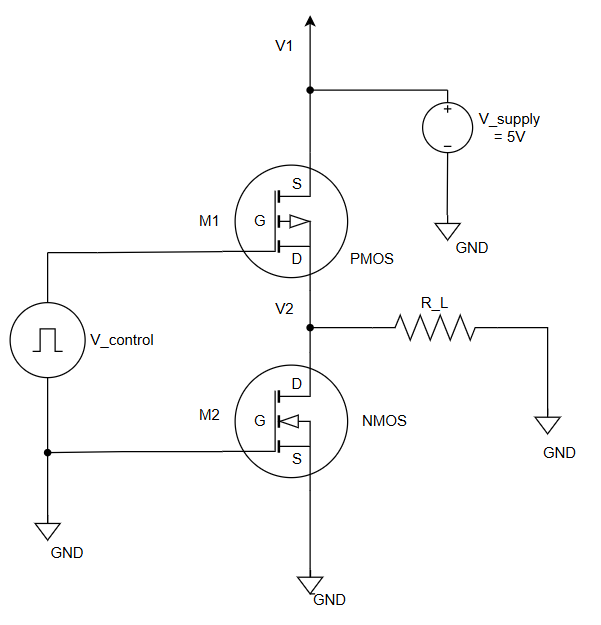
\includegraphics[width=0.5\linewidth]{Screenshot 2026-02-28 235603.png}
    \end{figure}

    \begin{figure}[H]
        \centering
        \caption{LTspice schematics of switch type 1}
        \vspace{0.3cm}
        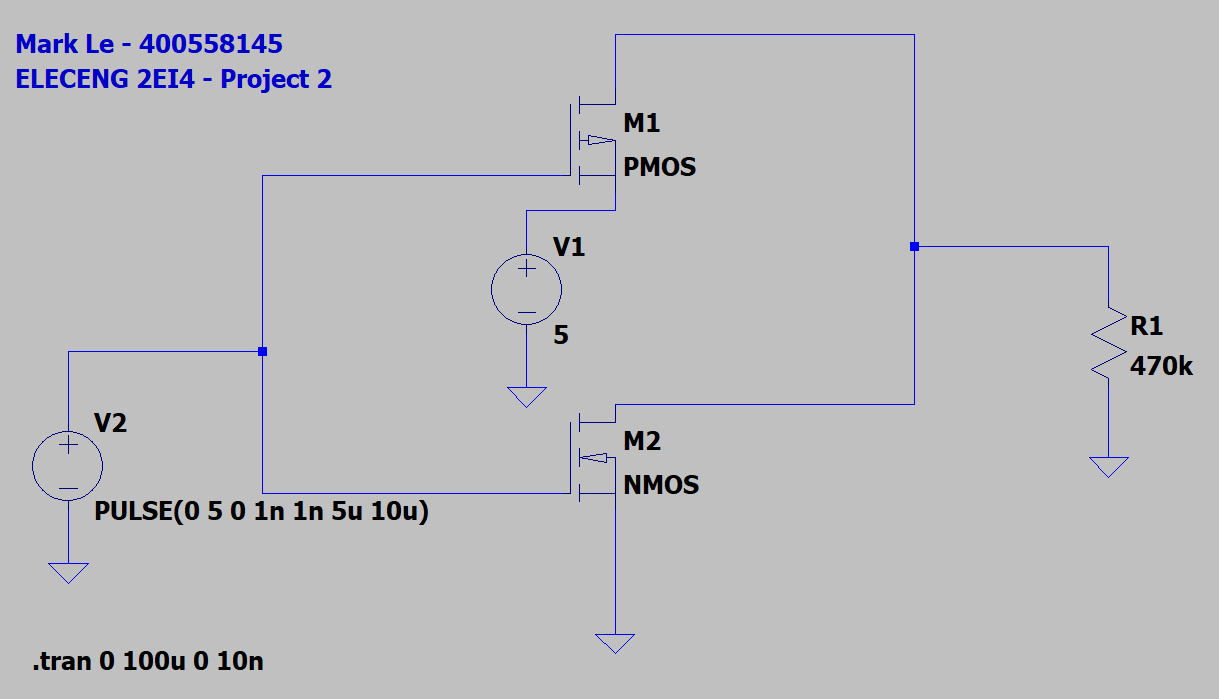
\includegraphics[width=0.8\linewidth]{Screenshot 2026-03-02 142817.png}
    \end{figure}

    \subsection{Measurement Performation}

    Here is the LTspice plot: 
 
    
    \begin{figure}[H]
        \centering
        \caption{LTspice plot of \(V_{control}\) (green), \(V_{out}\) (red), \(V_{supply}\) (blue)}
        \vspace{0.3cm}
        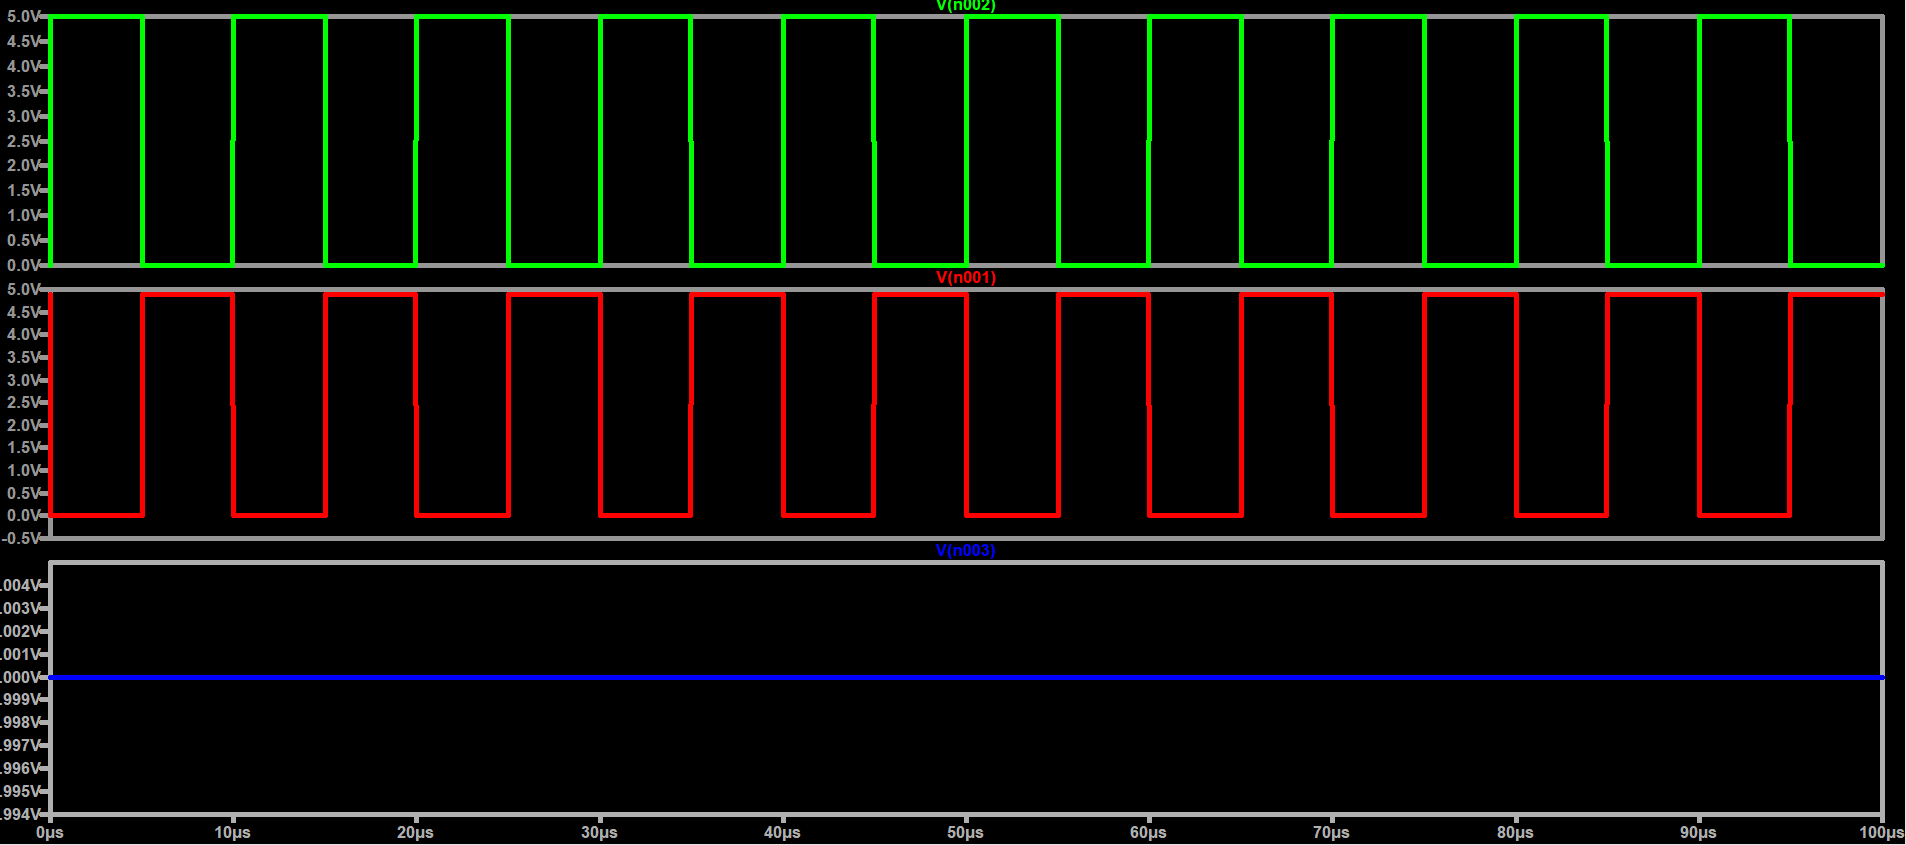
\includegraphics[width=1.1\linewidth]{Screenshot 2026-03-02 184420.png}
    \end{figure}

    
    Here is the experiment on the AD3:

    \begin{figure}[H]
        \centering
        \caption{Circuit built on the breadboard with the physical MOSFET IC chip (CD4007CN)}
        \vspace{0.3cm}
        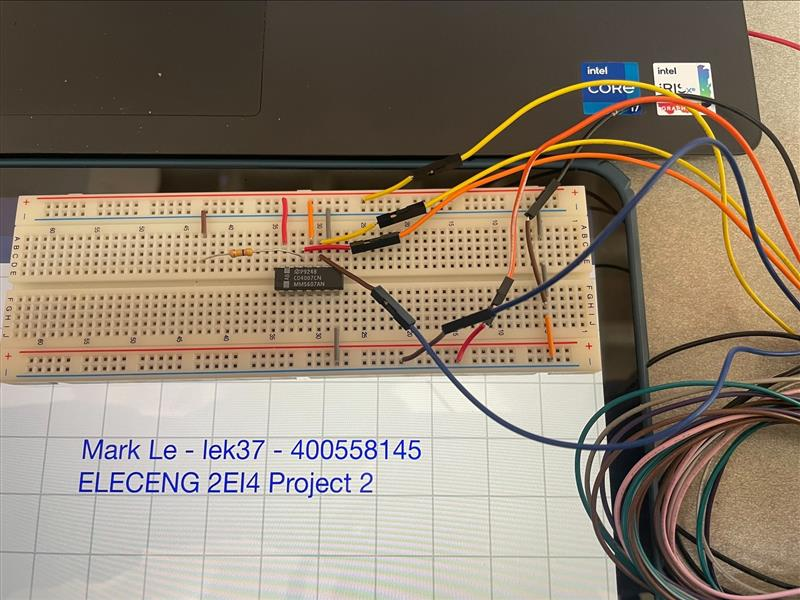
\includegraphics[width=0.75\linewidth]{Image (3).jpg}
    \end{figure}

    \newpage
    AD3 Waveform measurement results:

    \begin{figure}[H]
        \centering
        \caption{Wavegen setup for \(V_{control}\) and \(V_{supply}\):}
        \vspace{0.3cm}
        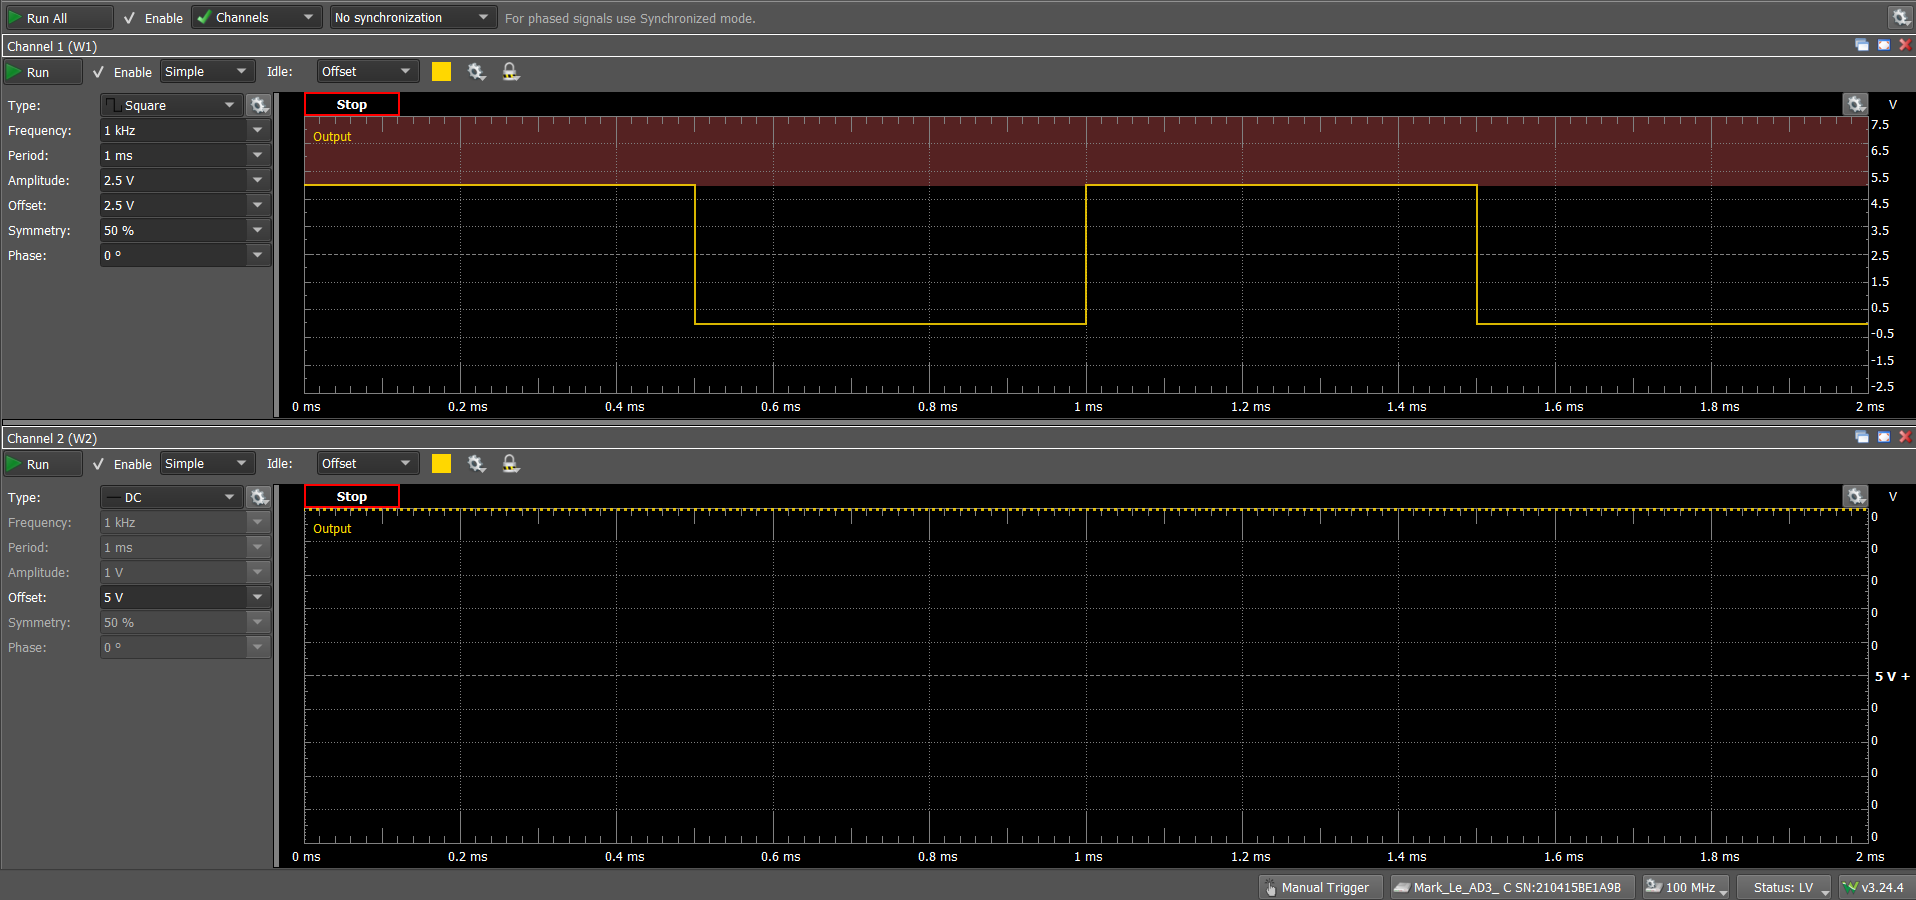
\includegraphics[width=1\linewidth]{Screenshot 2026-03-02 145947.png}
    \end{figure}


    \begin{figure}[H]
        \centering
        \caption{Measurement results of \(V_{out}\) (or \(V_2\)) compared to \(V_{control}\)}
        \vspace{0.3cm}
        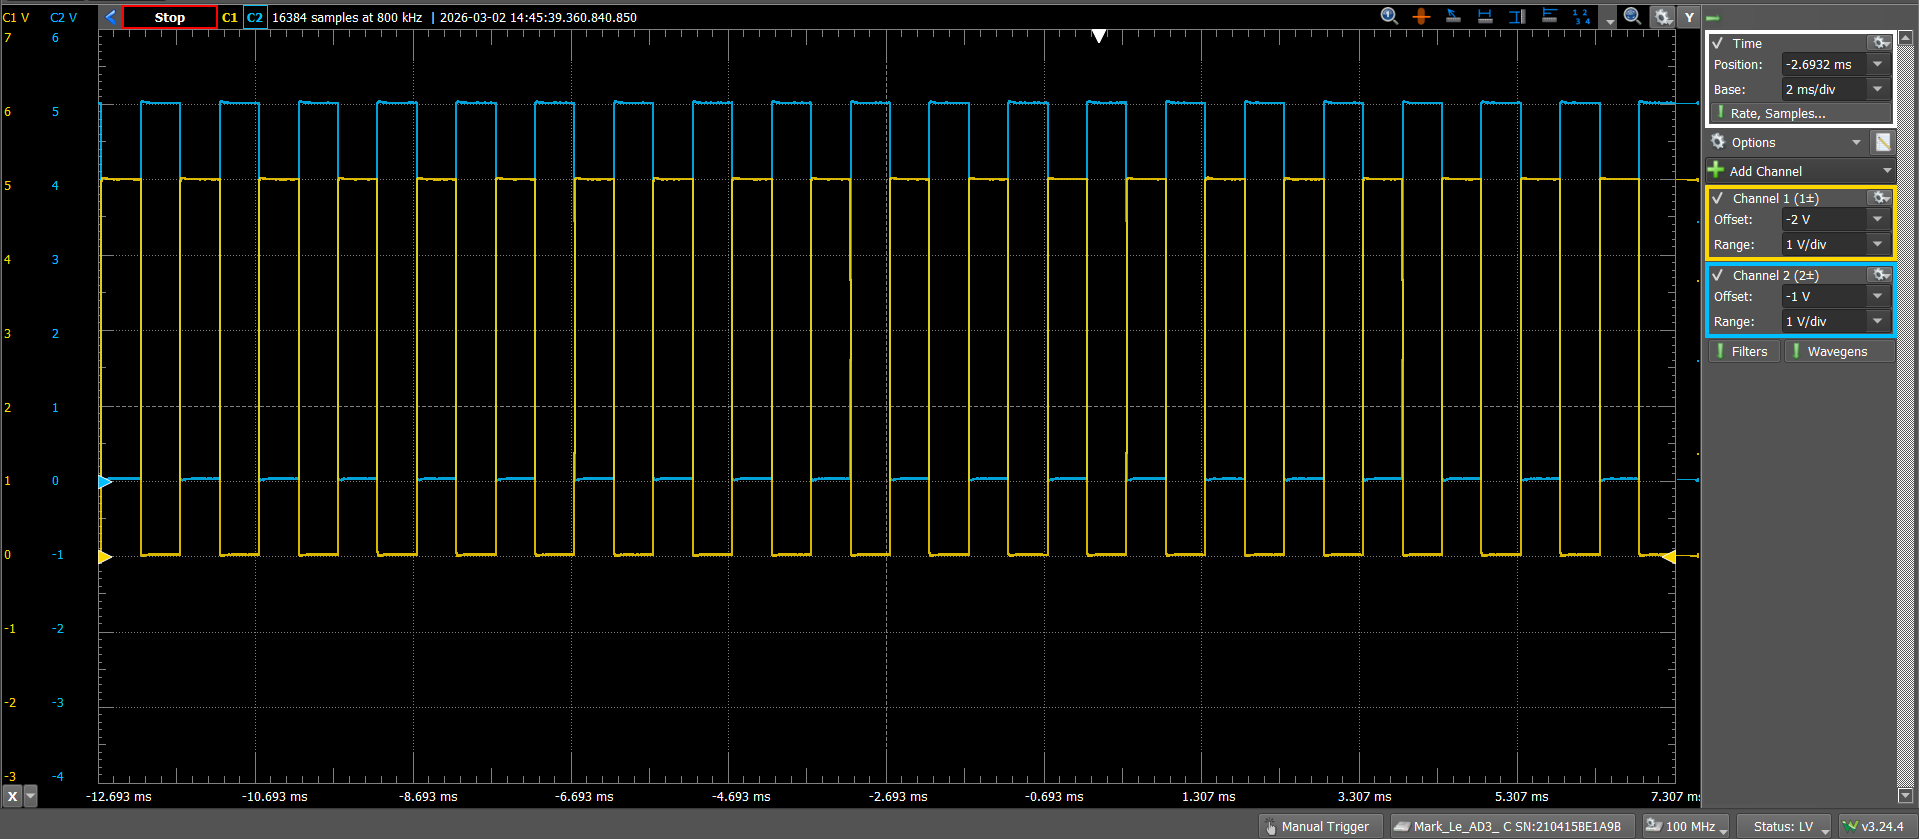
\includegraphics[width=1\linewidth]{Screenshot 2026-03-02 150308.png}
    \end{figure}

    For readability, I adjusted the offset of 2 waveform to be different with each other. 

    \newpage
    \textbf{Theoretical Calculation:}

    The threshold voltage \(V_T\) and the trans-conductance parameter \(k\) of the CD4007CN IC is given as the following:
    
    \begin{itemize}
        \item PMOS: \(V_T=1.7 V\), \(k=4.4 \mu A/V^2\)
        \item NMOS: \(V_T=1.75 V\), \(k=7.3 \mu A/V^2\)
    \end{itemize}

    \begin{tcolorbox}[title = Voltage drop when the switch is closed (ON state)]
        \(V_{control} = 0V\)


        For the NMOS (M2), we know that: \(V_{GS2}=V_{G2}-V_{S2}=V_{control}-0V=0V\)


        \(\therefore\) \(V_{GS2} < V_T\) \(\Rightarrow\) NMOS must be in cutoff \(\Rightarrow I_{DS2}=0A\)


        For the PMOS (M1), we know that \(V_{SG1}=V_{S1}-V_{G1}=5V-V_{control}=5V-0V=5V\)


        \(\therefore\) \(V_{SG1}>-V_T\) (\(V_T=-1.7V\)) \(\Rightarrow\) PMOS is in either linear or saturation mode. 


        Assuming the PMOS is in linear mode 


        \(\Rightarrow I_{SD1}=\frac{k}{2}[(V_{SG1}+V_{T1})V_{SD1}-\frac{V_{DS1}^2}{2}]\) 

        On the other hand, \(I_{SD1}=\frac{V_2}{R_L}=\frac{5-V_{SD1}}{470k}\)

        Equating both side, we got \(V_{SD1}=0.705 V\)


        By checking the region, we got \(V_{SD1}<V_{SG1}+V_T\), so the PMOS is indeed in linear mode. Therefore, \(V_{drop} \approx 0.705V\)

        

    \end{tcolorbox}

    \begin{tcolorbox}[title = Current leakage when the switch is opened (OFF state)]
        \(V_{control}=5V\)


        \(V_{SG1}=V_{S1}-V_{G1}=V_1-V_{control}=5V-5V=0V\)


        \(\therefore\) \(V_{SG1} < -V_{T1} \) (\(V_{T1}=-1.7V\)). Therefore the PMOS has to be in cutoff and \(I_{SD1}=0\) A (no current leakage). 
    \end{tcolorbox}

    \newpage
    \textbf{Experimental Measurements}

    \begin{figure}[H]
        \centering
        \caption{Measurement of \(V_2\) with cursor placed at when the switch is ON/OFF}
        \vspace{0.3cm}
        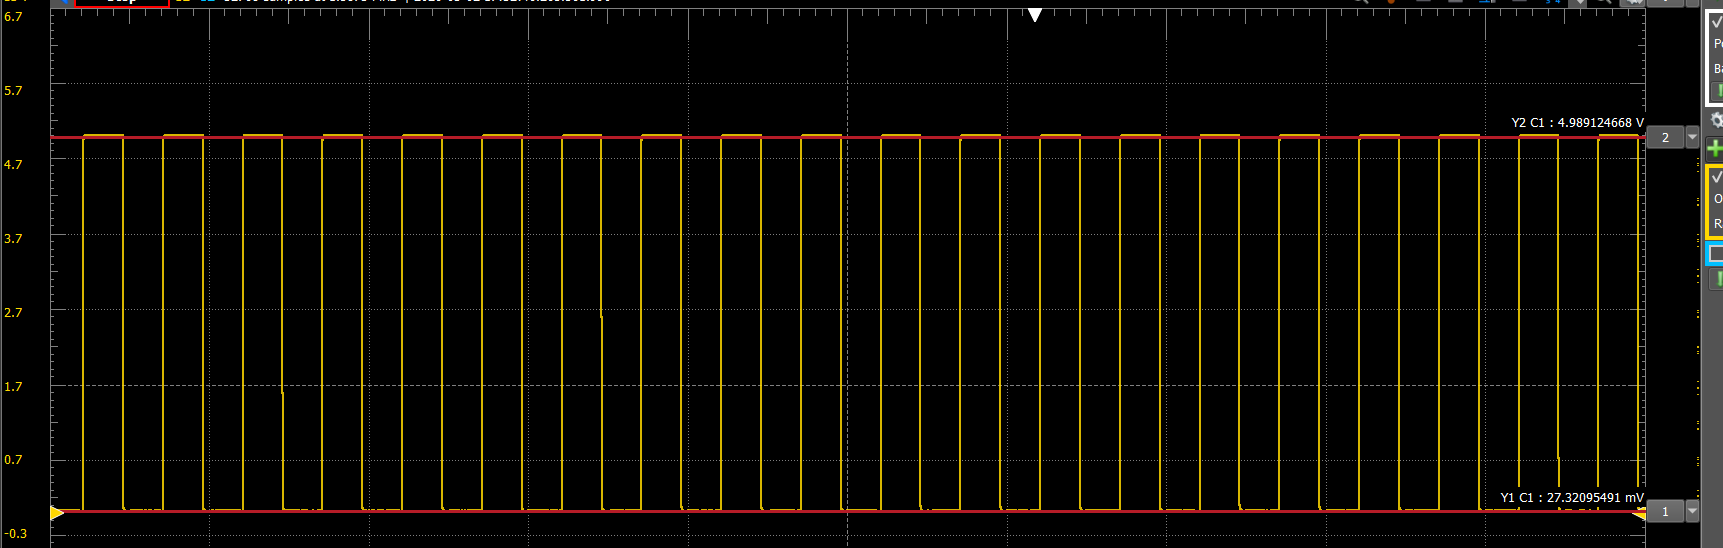
\includegraphics[width=1\linewidth]{Screenshot 2026-03-02 180901.png}
    \end{figure}
    
    \begin{itemize}
        \item Voltage drop when the switch is closed (\(V_{control}=0V\)): \(V_{12}=V_1-V_2=V_{S1}-V_{D1}=5V-4.989V=0.011V\)
        \item Current leak when the switch is opened (\(V_{control}=5V\): \(I_{L}=V_2/R_L=27.32 mV/470k \Omega=5.81 \times 10^{-5}\) mA
    \end{itemize}

    

    \subsection{Theoretical Explaination:}

    Based on the result, it can be seen that the experimental voltage drop was small, at 0.011 V, which is a lot better than the theoretical calculation, but a bit worse than the simulation, as LTspice simulation suggests that almost no voltage drop should happen. Additionally, even though the current leakage was very small, it is still exist with a value of \(5.81 \times 10^{-5}\) mA, thus imply that this MOSFET-based switch is definitely not an ideal switch, as ideal switch requires the voltage drop and the current leakage has to be 0V/0A. 
    
    \subsection{Design Tradeoffs}

    One of the biggest design trade-offs while implementing this switch is the limitation of the components. The design was only able to use a resistor, 2 MOSFETs and the AD3 wavegen/power supply, resulting in a economic-friendly switch, and the result is obviously could not be better than a more expensive switch. A bigger resistor could have been used, but the \(470k\Omega\) is the maximum that can be obtained from the 2CI4/2EI4 kit. 



    \newpage

    \begin{thebibliography}{9}
        \bibitem{Analog Dialogue}
        ADI Analog Dialogue, ``ADALM2000 Activity: Build CMOS Logic Functions Using the CD4007 Array'' 
        [Online]. Available: https://www.analog.com/en/resources/analog-dialogue/studentzone/studentzone-september-2022.html Accessed Mar 1. 2026.
    \end{thebibliography}

    

    
\end{document}